\documentclass[10pt]{article}

\usepackage{epsilonj}

\usepackage{tikz}
\usetikzlibrary{calc,intersections,decorations.pathreplacing} 
\usetikzlibrary{arrows.meta}
% этот код считает отмечает углы в tikz
\newcommand\markangle[6]{% origin X Y radius radiusmark mark
  % fill red circle
  \begin{scope}
    \path[clip] (#1) -- (#2) -- (#3);
    \fill[color=red,fill opacity=0.5,draw=red,name path=circle]
    (#1) circle (#4);
  \end{scope}
  % middle calculation
  \path[name path=line one] (#1) -- (#2);
  \path[name path=line two] (#1) -- (#3);
  \path[%
  name intersections={of=line one and circle, by={inter one}},
  name intersections={of=line two and circle, by={inter two}}
  ] (inter one) -- (inter two) coordinate[pos=.5] (middle);
  % put mark
  \node at ($(#1)!#5!(middle)$) {#6};
}

\RequirePackage{graphicx}
\RequirePackage[colorlinks,citecolor=blue,urlcolor=blue]{hyperref}

\newcommand{\specialcell}[2][c]{\begin{tabular}[#1]{@{}c@{}}#2\end{tabular}}
\newcommand{\RR}{\mathbb{R}}

\begin{document}

\TITLE{Корреляция: простая, частная и условная}
\SHORTTITLE{Корреляция: простая, частная и условная}

\AUTHOR{Борис Демешев}{НИУ ВШЭ, Москва.}
\SHORTAUTHOR{Борис Демешев}

\DoFirstPageTechnicalStuff


\newtheorem{theorem}{Теорема}
\newtheorem{definition}{Определение}

\begin{abstract}
Корреляция "--- это способ описать силу линейной зависимости между двумя случайными величинами одним числом. Каков геометрический смысл корреляции? Что такое частная корреляция? Как связаны частная и условная корреляция? 
\end{abstract}

\begin{keyword}
корреляция, частная корреляция, условная корреляция, косинус, проекция
\end{keyword}



\section{Корреляция по-русски}

Обычно в учебниках даётся такое определение корреляции

\begin{equation}
\label{def_corr}
\Corr(X,Y)=\frac{\Cov(X,Y)}{\sqrt{\Var(X)\Var(Y)}}.
\end{equation}

Естественно, возникает вопрос: «С какого перепугу? Почему это мы делим ковариацию на что-то там?»

Мы дадим определение корреляции словами:

\begin{definition}
Корреляция между случайными величинами $X$ и $Y$ показывает на сколько своих стандартных отклонений в среднем растёт случайная величина $Y$ при росте случайной величины $X$ на одно своё стандартное отклонение.
\end{definition}

А теперь из этого словесного определения мы получим формулу \ref{def_corr}. Разложим величину $Y$ на два слагаемых. Первое слагаемое вбирает в себя всю ту часть $Y$, которая линейно зависит от $X$, а второе "--- всё оставшееся:

\[
\frac{Y}{\sigma_Y}=\rho \cdot \frac{X}{\sigma_X} + \varepsilon
\]

В этой формуле видно, что с ростом $X$ на одно стандартное отклонений $\sigma_X$ правая часть изменится в среднем на $\rho$, и, следовательно, величина $Y$ в среднем изменится на $\rho \cdot \sigma_Y$. 

%\[
%Y=\beta \cdot X + \varepsilon
%\]
%
%Здесь $\beta$ показывает на сколько единиц в среднем растёт $Y$ при росте $X$ на одну единицу. 

Мы хотим, чтобы ... $\Cov(X,\varepsilon)=0$. 


\[
\Cov\left(X, \frac{Y}{\sigma_Y} - \rho \cdot \frac{X}{\sigma_X} \right) = 0
\]

По свойствам ковариации получаем

\[
\Cov(X,Y)/\sigma_Y- \rho \Cov(X,X)/\sigma_X=0
\]

И, тадам, выражаем корреляцию, $\rho$:

\[
\rho = \frac{\Cov(X,Y)/\sigma_Y}{\Cov(X,X)/\sigma_X} = \frac{\Cov(X,Y)}{\sigma_X \sigma_Y}
\]

Несмотря на асимметричность исходного разложения (эпсилон прибавляется в правой части уравнения к величине $X$), результирующая формула для корреляции получается симметричной. Из этого следует, что ровно такой же результат получится, если начать с разложения:
\[
\frac{X}{\sigma_X}=\rho \cdot \frac{Y}{\sigma_Y} + \varepsilon
\]

Из определения неочевидно, что корреляция лежит в пределах от $-1$ до $1$. ...


Стоит обратить внимание на немного контр-интуитивный факт. Если бы зависимость между $X$ и $Y$ была бы жесткой детерминистической, и с ростом $X$ на единицу величина $Y$ росла бы на $\Delta$, то с ростом $Y$ на единицу величина $X$ росла бы на $1/\delta$. Для случайных величин обращения не происходит. Если с ростом $X$ на одно своё стандартное отклонение величина $Y$ в среднем растёт на $\rho$ своих стандартных отклонений, то и с ростом $Y$ на одно своё стандартное отклонение величина $X$ в среднем растёт на $\rho$ своих стандартных отклонений.



? парадокс возвращения к среднему ?


\section{Геометрический смысл корреляции}

Давайте рисовать случаные величины векторами-стрелочками! Не в том смысле, что у стрелочки случайное направление или длина, а в том смысле, что направление и длина стрелочки описывают характеристики этой случайной величины. 

Любую геометрию можно задать, задав скалярное произведение. Действительно, если мы умеем считать скалярное произведение двух любых векторов, $<\vec{a},\vec{b}>$, то длина вектора считается ровно как в 9-м классе:

\[
|\vec{a}|=\sqrt{<\vec{a},\vec{a}>}
\]

И также любой девятикласник помнит, что косинус угла между векторами считается как

\[
\cos(\vec{a},\vec{b})=\frac{<\vec{a},\vec{b}>}{|\vec{a}||\vec{b}|}
\]

Мы определим скалярное произведение двух случайных величин как их ковариацию:

\[
<X,Y>=\Cov(X,Y)
\]

При таком подходе длиной случайной величины окажется стандартное отклонение:

\[
\sqrt{\Cov(X,X)}=\sqrt{\Var(X)}=\sigma_X
\]

А корреляция окажется косинусом угла между случайными величинами:
\[
\cos \phi =\cos(X,Y)=\frac{\Cov(X,Y)}{\sigma_X\sigma_Y}=\Corr(X,Y)
\]


\begin{center}
\begin{tikzpicture}
\path (0,0) coordinate (origin);
\path (origin) ++(1,2) coordinate (Y);
\path (origin) ++(3,0) coordinate (X);
\draw[-{Latex[length=3mm]},thick] (origin) -- (Y);
\draw[-{Latex[length=3mm]},thick] (origin) -- (X);
\node [above] at (X) {$X$};
\node [right] at (Y) {$Y$};
\markangle{origin}{X}{Y}{6mm}{4mm}{$\phi$}
\end{tikzpicture}
\end{center}

Значит в нашей геометрии  длина стрелочки "--- стандартное отклонение случайной величины, а косинус угла между двумя стрелочками "--- это корреляция двух случайных величин. Дисперсия, следовательно, это квадрат длины случайной величины. Перпендикулярными случайными величинами будут те, косинус угла между которыми равен нулю, то есть некоррелированные.

Например, сформулируем в данной геометрии теорему Пифагора. Если случайные величины $X$ и $Y$ перпендикулярны (корреляция или ковариация равны нулю), то дисперсия их суммы (квадрат длины гипотенузы) равен сумме их дисперсий (сумму квадратов длин катетов):

\[
\Var(X+Y)=\sigma^2_{X+Y}=\sigma^2_X+\sigma^2_Y=\Var(X)+\Var(Y)
\]

\begin{center}
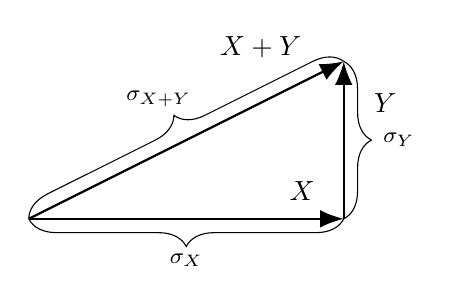
\begin{tikzpicture}
\path (0,0) coordinate (origin);
\path (origin) ++(4,2) coordinate (Y);
\path (origin) ++(4,0) coordinate (X);
\draw[-{Latex[length=3mm]},thick] (origin) -- (Y);
\draw[-{Latex[length=3mm]},thick] (origin) -- (X);
\draw[-{Latex[length=3mm]},thick] (X) -- (Y);
\node [yshift=10pt,xshift=-15pt] at (X) {$X$};
\node [yshift=-15pt,xshift=15pt] at (Y) {$Y$};
\node [yshift=5pt,xshift=-30pt] at (Y) {$X+Y$};
\draw [decorate,decoration={brace,amplitude=10pt}] (X) -- (origin) node [black,midway,yshift=-15pt] {\footnotesize $\sigma_X$};
\draw [decorate,decoration={brace,amplitude=10pt}] (Y) -- (X) node [black,midway,xshift=20pt] {\footnotesize $\sigma_{Y}$};
\draw [decorate,decoration={brace,amplitude=10pt}] (origin) -- (Y) node [black,midway,yshift=15pt,xshift=-10pt] {\footnotesize $\sigma_{X+Y}$};
\end{tikzpicture}
\end{center}

Введение геометрии позволяет говорить о проекции. Например, можно спроецировать случайную величину $Y$ на множество случайных величин пропорциональных величине $X$, $\{cX | c\in \RR \}$. Если на обычной плоскости спроецировать вектор $\vec{a}$ на прямую, порожденную вектором $\vec{b}$, то получится $\cos(\vec{a},\vec{b})\cdot \vec{b}$. По аналогии, если спроецировать случайную величину $Y$ на множество $\{cX | c\in \RR \}$, то получится $\Corr(X,Y)\cdot X$. Другими словами, среди случайных величин пропорциональных $X$ величина  $\Corr(X,Y)\cdot X$ --- самая похожая на величину $Y$.



\section{Корреляция и независимость}

\begin{theorem}
Случайные величины $X$ и $Y$ независимы тогда и только тогда, когда некоррелированы любые функции $f(X)$ и $g(Y)$.
\end{theorem}

Другими словами для независимости $X$ и $Y$ необходима некоррелированность пар $X$ и $Y$, $X^2$ и $\cos(Y)$, $\exp(X)$ и $1/Y$, и так далее. Из этого следует, что некоррелированность $X$ и $Y$ является необходимым, но недостаточным условием для независимости.

Многие ошибочно считают, что если величина $X$ имеет нормальное распределение $N(\mu_X, \sigma^2_X)$ и величина $Y$ имеет нормальное распределение $N(\mu_Y, \sigma^2_Y)$, и $X$ и $Y$ некоррелированы, то они независимы. Это неверно.

Контрпример. Случайная величина $X$ имеет стандартное нормальное распределение $N(0;1)$, случайная величина $Z$ независима от $X$ и равновероятно принимает значения $-1$ и $+1$. Определим величину $Y$ как их произведение, $Y=XZ$. 

В этом примере величины $X$ и $Y$ зависимы, так как $|X|=|Y|$. Однако $Y$ распределена нормально стандартно и $\Corr(X,Y)=0$.  

Правильная теорема звучит так:

\begin{theorem}
Если некоррелированные случайные величины $X$ и $Y$ имеют совместное нормальное распределение, то $X$ и $Y$ независимы.
\end{theorem}

Попутно упомянем ещё одно неожиданное свойство предъявленного контрпримера. Если случайные величины нормальны по отдельности, то вполне возможно, что их сумма ненормальна. Для пары величин, имеющих совместное нормальное распределение, это невозможно.


\section{Частная корреляция}

\begin{definition}
Частная корреляция между величинами $X$ и $Y$ при фиксированной величине $Z$ показывает на сколько своих стандартных отклонений $\sigma_Y$ в среднем вырастет $Y$ при росте величины $X$ на одно своё стандартное отклонение $\sigma_X$ и постоянном значении величины $Z$.
\end{definition}

Для нахождения частной корреляции используется разложение
\[
\frac{Y}{\sigma_Y}=\rho_{XY|Z} \cdot \frac{X}{\sigma_X} + \rho_{YZ|X} \frac{Z}{\sigma_Z} + \varepsilon
\]


Альтернативный подход к подсчёту частной корреляции следующий:
\begin{enumerate}
\item Спроецируем $X$ на множество величин, некоррелированных с $Z$. Получим $\tilde{X}$.
\item Спроецируем $Y$ на множество величин, некоррелированных с $Z$. Получим $\tilde{Y}$.
\item Частная корреляция между $X$ и $Y$ при фиксированной $Z$ "--- это обычная корреляция между $\tilde{X}$ и $\tilde{Y}$.
\end{enumerate}


(картинка ...)


Два подхода к определению частной корреляции эквивалентны в силу теоремы Фриша-Ву-Ловелла (Frisch–Waugh–Lovell). Обычно эта теорема формулируется применительно к регрессии, а здесь мы приведём её вариат для случайных величин.

\begin{theorem}
Если имеют место разложения:
\[
Y=a_1 Z_1 + a_2 Z_2 + \ldots + a_n Z_n + \tilde{Y}, \text{ где }\; \tilde{Y}\bot Z_1, Z_2, \ldots, Z_n
\]
и
\[
X=b_1 Z_1 + b_2 Z_2 + \ldots + b_n Z_n  + \tilde{X}, \text{ где }\; \tilde{X}\bot Z_1, Z_2, \ldots, Z_n
\]
То в разложениях  
\[
\tilde{Y}=d \tilde{X} + \varepsilon, \text{ где }\; \varepsilon \bot \tilde{X}
\]
и
\[
Y=c_1 Z_1 + c_2 Z_2 + \ldots + c_n Z_n  + dX + u, \text{ где }\; u \bot Z_1, Z_2, \ldots, Z_n, X
\]
коэффициенты при $\tilde{X}$ и $X$ совпадают.
\end{theorem}



\section{Условная корреляция}

\begin{definition}
Условная корреляция между величинами $X$ и $Y$ при известном значении величины $Z$ показывает на сколько своих стандартных отклонений $\sigma_Y$ в среднем вырастет $Y$ при росте величины $X$ на одно своё стандартное отклонение $\sigma_X$ при заданном значении величины $Z$.
\end{definition}


Следует подчеркнуть одно существенное отличие условной корреляции от обычной и частной. Обычная и частная корреляция являеются константами. Условная корреляция $\Corr(X,Y|Z)$ является функцией от $Z$. Величина $Z$ является случайной, поэтому и условная корреляция $\Corr(X,Y|Z)$ является случайной величиной. 

Здесь регрессионное определение???? 

Чуть более формальное определение:

\begin{definition}
\[
\Corr(X,Y|Z) = \frac{\Cov(X,Y|Z)}{\sqrt{\Var(X|Z)\Var(Y|Z)}},
\]
\end{definition}

где $\Cov(X,Y|Z)=\E(XY|Z)-\E(X|Z)\E(Y|Z)$ и $\Var(X|Z)=\E(X^2|Z)-(\E(X|Z))^2$


Пример подсчета частной и условной корреляций.

\begin{theorem}
Если величины $X$, $Y$ и $Z$ имеют совместное нормальное распределение, то частная и условная корреляции совпадают.
\end{theorem}

\end{document}


